\section{基本介绍}

\subsection{安装}

鼠标右键点击 \lstinline{install.ps1} 点击在 Powershell 中运行,完成对 LUA 程序的配置。

\begin{figure}[H]
    \Centering
    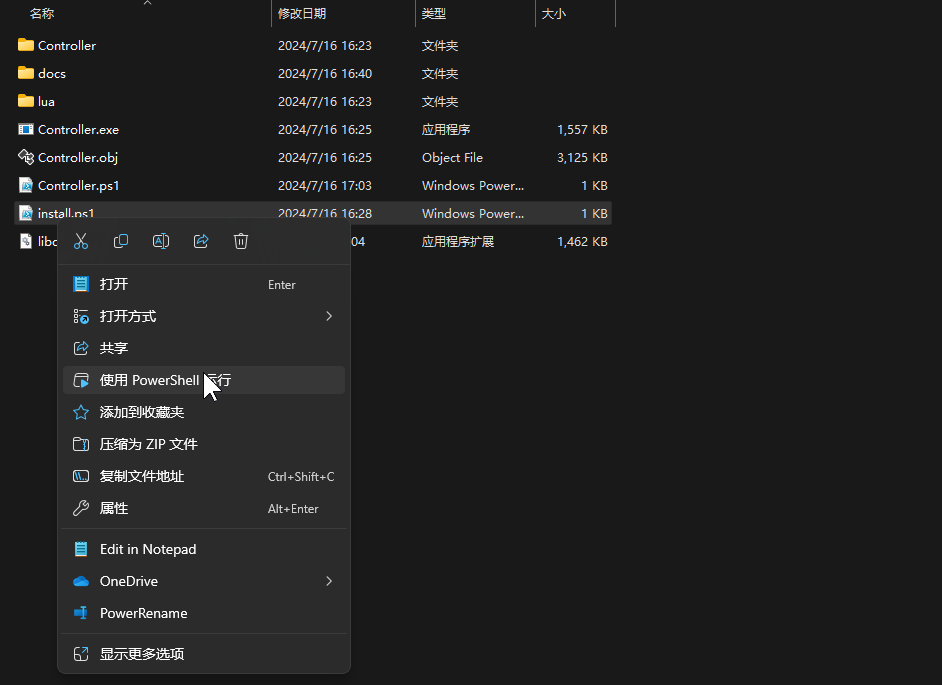
\includegraphics[width=\textwidth]{docs/assets/install.png}
    \caption{运行 install.ps1}
\end{figure}

本集成工具分为控制器 \lstinline{Controller} 和 LUA 源文件(保存于 \lstinline{lua} 目录下) 。

控制器\textbf{必须}以管理员权限启动(对计算机不熟悉的 \textbf{建议}按下图方式运行 \lstinline{Controller.ps1} 而非直接运行 \lstinline{Controller.exe} 本体),否则会因为权限不足导致无法正常使用断线重连功能(启动游戏需要管理员权限)。
控制器通过实时下达命令,控制集成工具的运行。

\begin{figure}[H]
    \Centering
    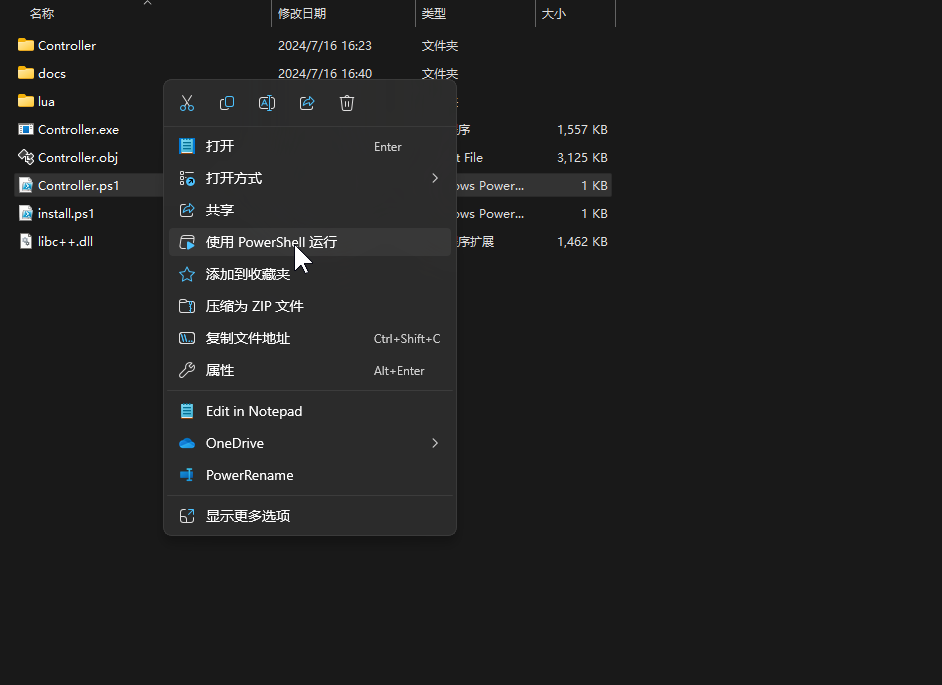
\includegraphics[width=\textwidth]{docs/assets/runas.png}
    \caption{以管理员身份启动}
\end{figure}

控制器在 Windows 控制台中运行,在控制台界面中按下 \lstinline{Ctrl} \lstinline{C}(推荐)或直接点击右上角关闭按钮可终止程序。

本节主要介绍控制器的基本使用、罗技 LUA 代码导入、集成工具的即时中断功能。

\begin{figure}[H]
    \Centering
    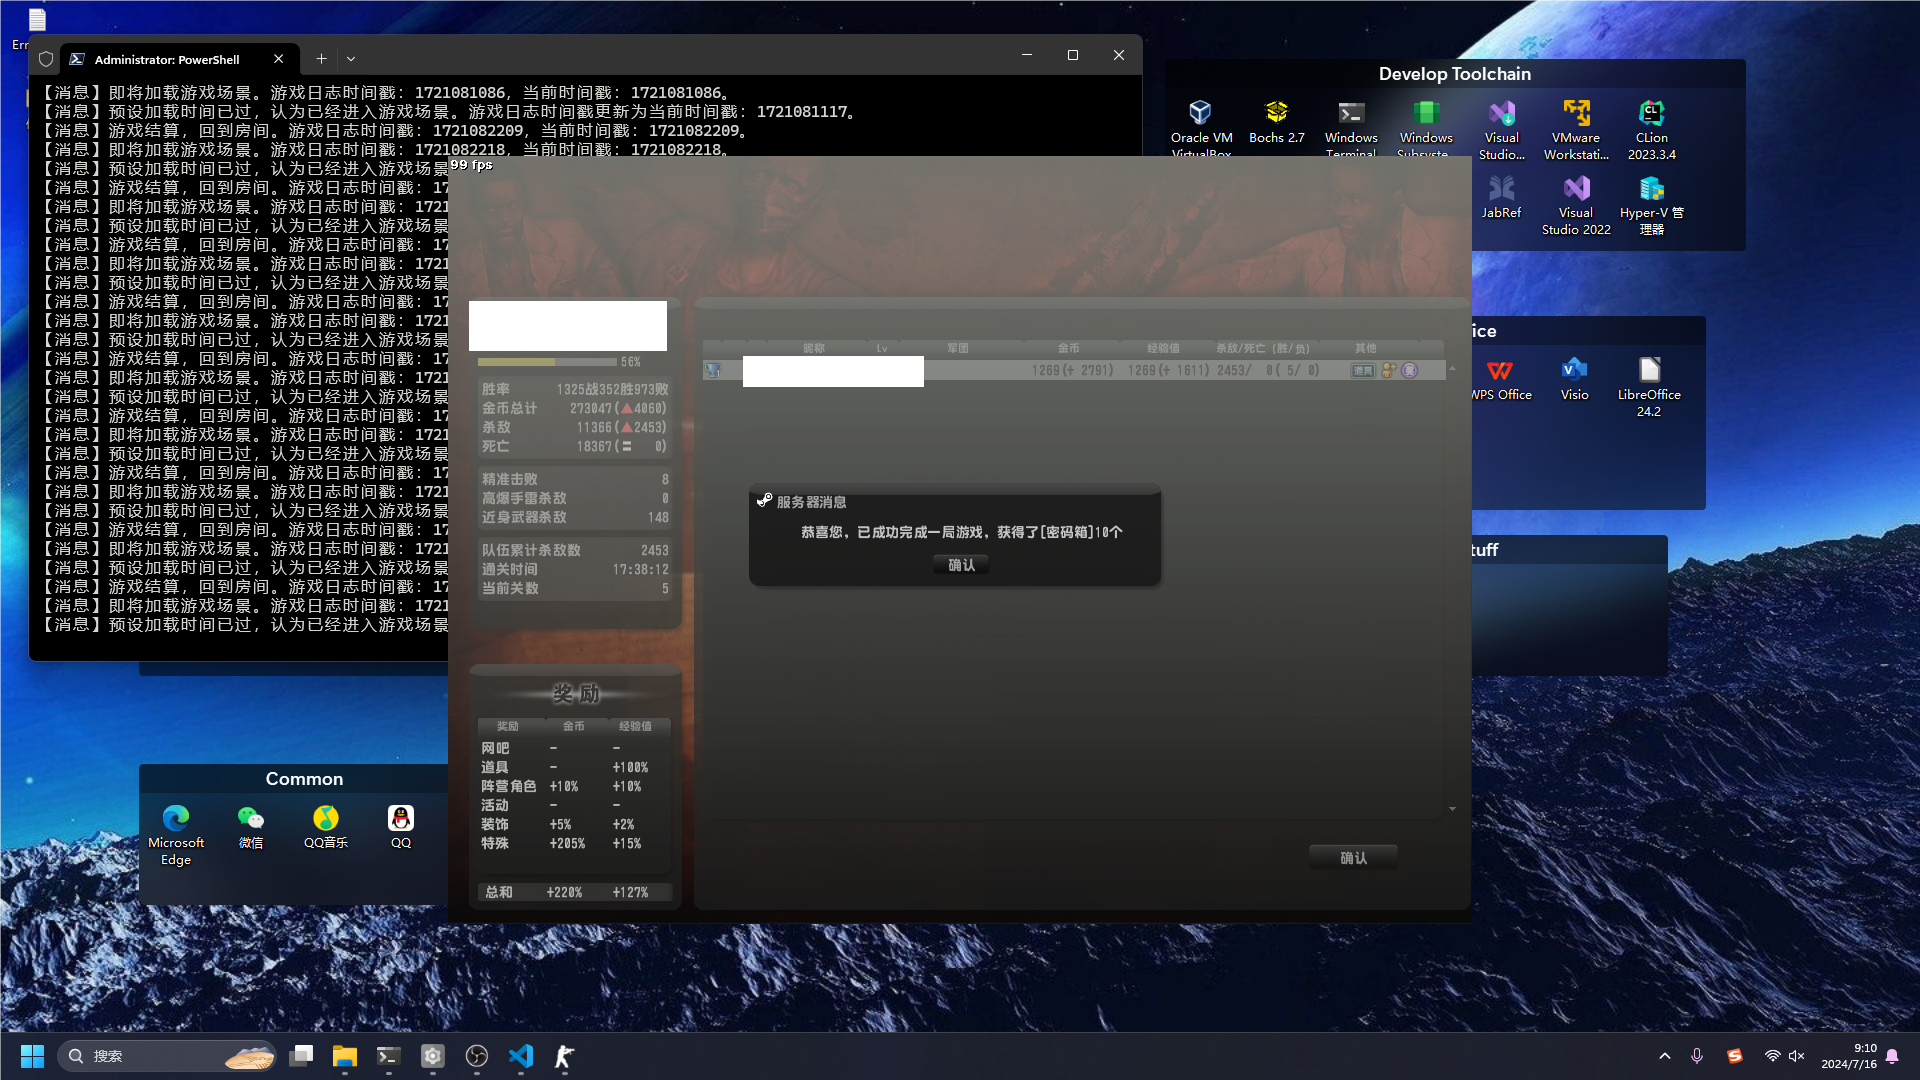
\includegraphics[width=\textwidth]{docs/assets/controller.png}
    \caption{\lstinline{Controller} 运行效果展示}
\end{figure}

\subsection{功能热键}

启动控制器后,会注册如下热键:

\begin{itemize}

    \item 0 模式:\lstinline{Ctrl} \lstinline{Alt} \lstinline{Shift} \lstinline{0},默认模式,该模式下不进行任何操作。

    \item 1 模式:\lstinline{Ctrl} \lstinline{Alt} \lstinline{Shift} \lstinline{1},单武器挂机模式。

    \item 2 模式:\lstinline{Ctrl} \lstinline{Alt} \lstinline{Shift} \lstinline{2},随机武器挂机模式。

    \item 3 模式:\lstinline{Ctrl} \lstinline{Alt} \lstinline{Shift} \lstinline{3},自动合成配件。

    \item 4 模式:\lstinline{Ctrl} \lstinline{Alt} \lstinline{Shift} \lstinline{4},自动重复购买同一件商店物品,可用于批量购买金币道具。

    \item 5 模式:\lstinline{Ctrl} \lstinline{Alt} \lstinline{Shift} \lstinline{5},定位坐标,将结果输出到罗技控制台。

\end{itemize}

\subsection{罗技软件导入 LUA 程序}

无需罗技设备,安装并\textbf{以管理员权限}启动 Logitech G HUB 软件。

\begin{figure}[H]
    \Centering
    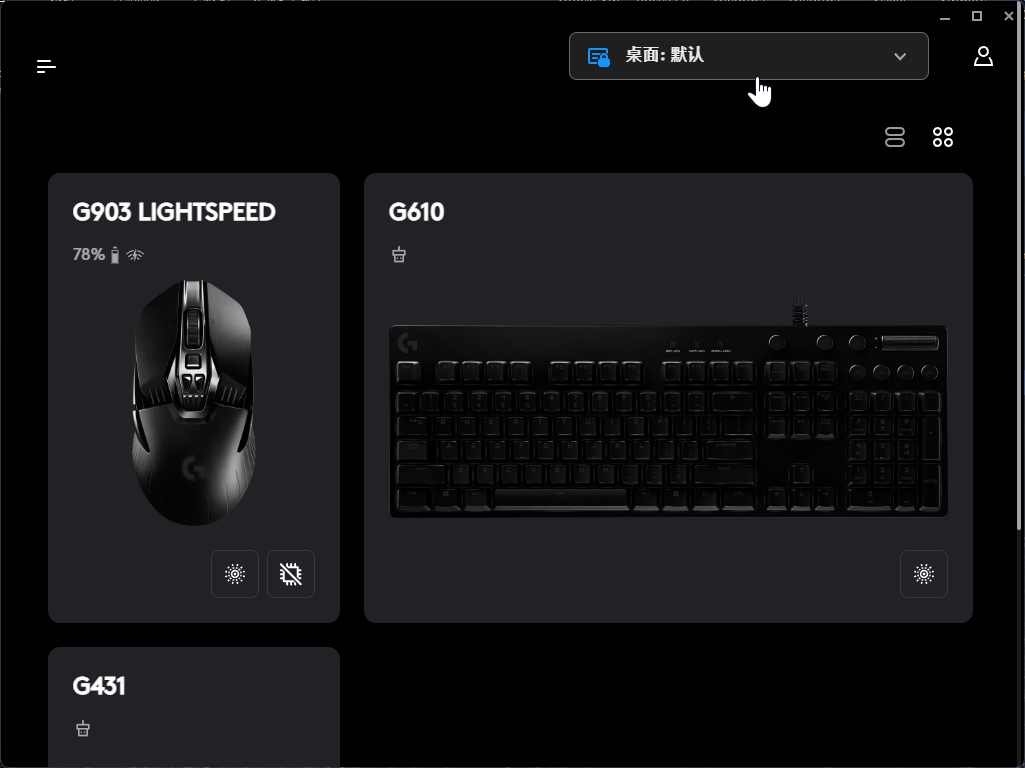
\includegraphics[width=\textwidth]{docs/assets/lghub.png}
    \caption{Logitech G HUB 软件}
\end{figure}

进入界面后,点击软件上方下拉框,选择“管理配置文件”。

\begin{figure}[H]
    \Centering
    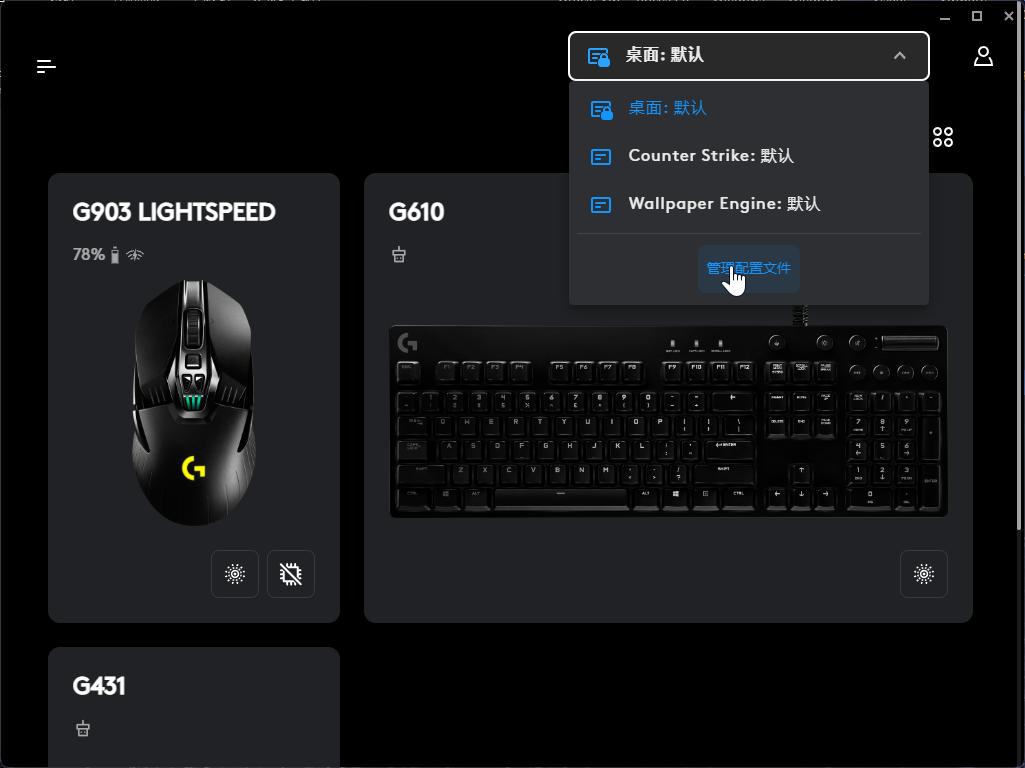
\includegraphics[width=\textwidth]{docs/assets/manage_configs.png}
    \caption{点击“管理配置文件”}
\end{figure}

在下一级界面中点击“编写脚本”。

\begin{figure}[H]
    \Centering
    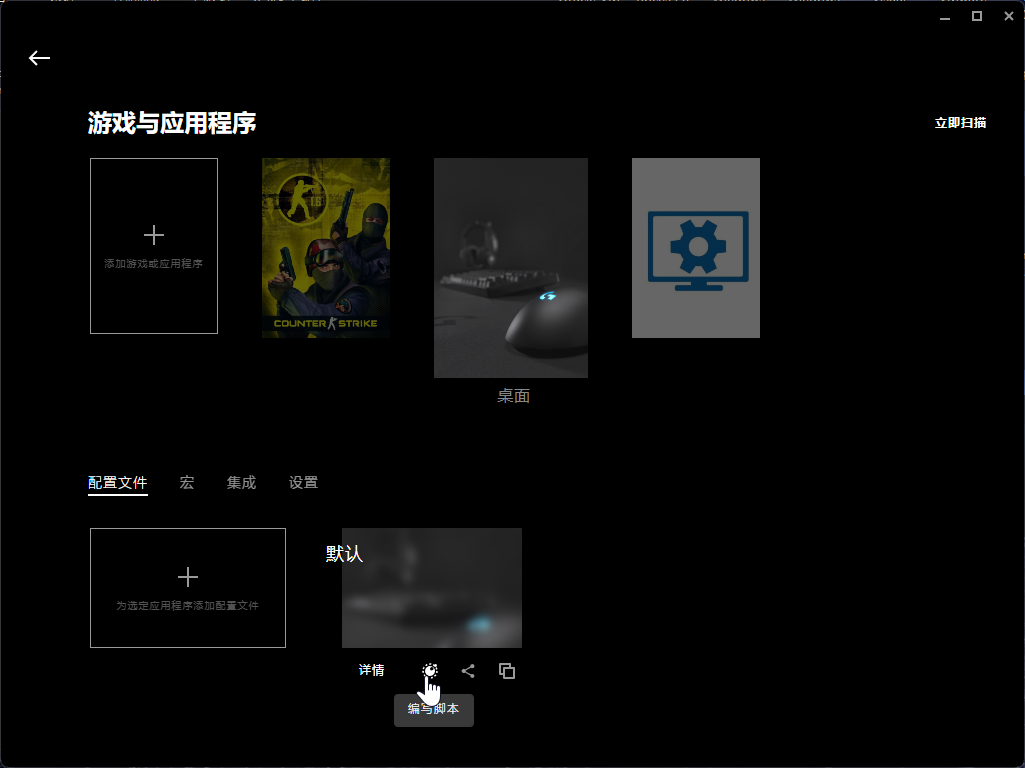
\includegraphics[width=\textwidth]{docs/assets/script.png}
    \caption{点击“编写脚本”}
\end{figure}

点击“脚本-导入”,将 LUA 源文件 \lstinline{main.lua} 导入软件,点击保存并运行(或直接按下 \lstinline{Ctrl} \lstinline{S})。

\begin{figure}[H]
    \Centering
    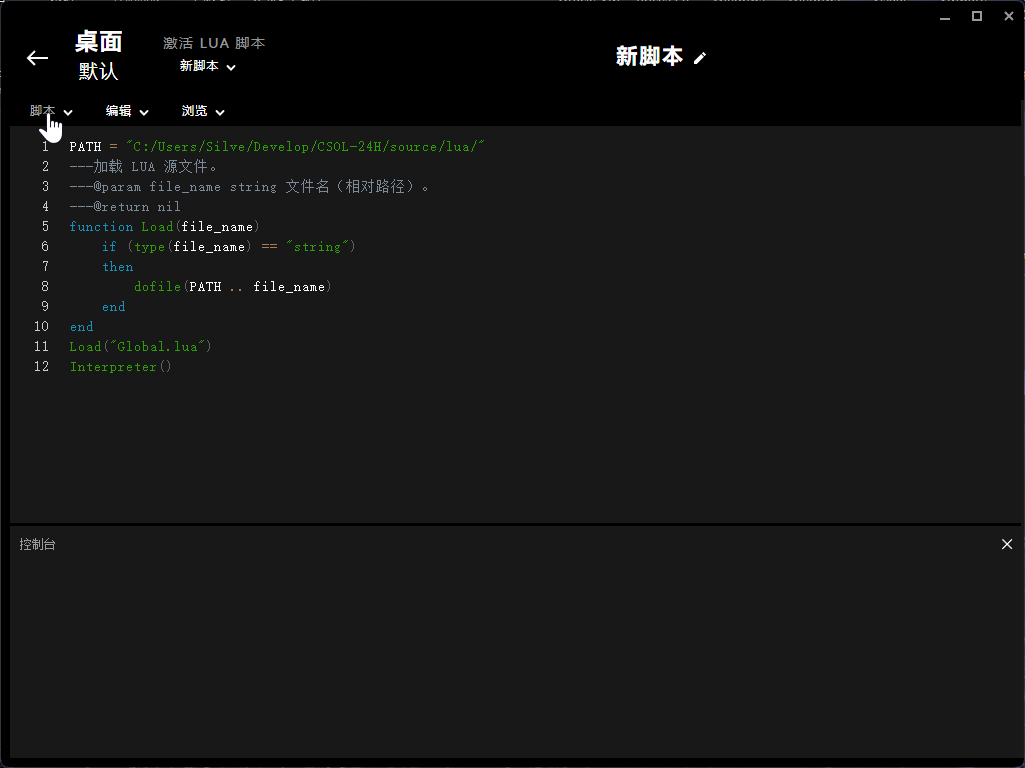
\includegraphics[width=\textwidth]{docs/assets/edit.png}
    \caption{点击“脚本”}
\end{figure}

\begin{figure}[H]
    \Centering
    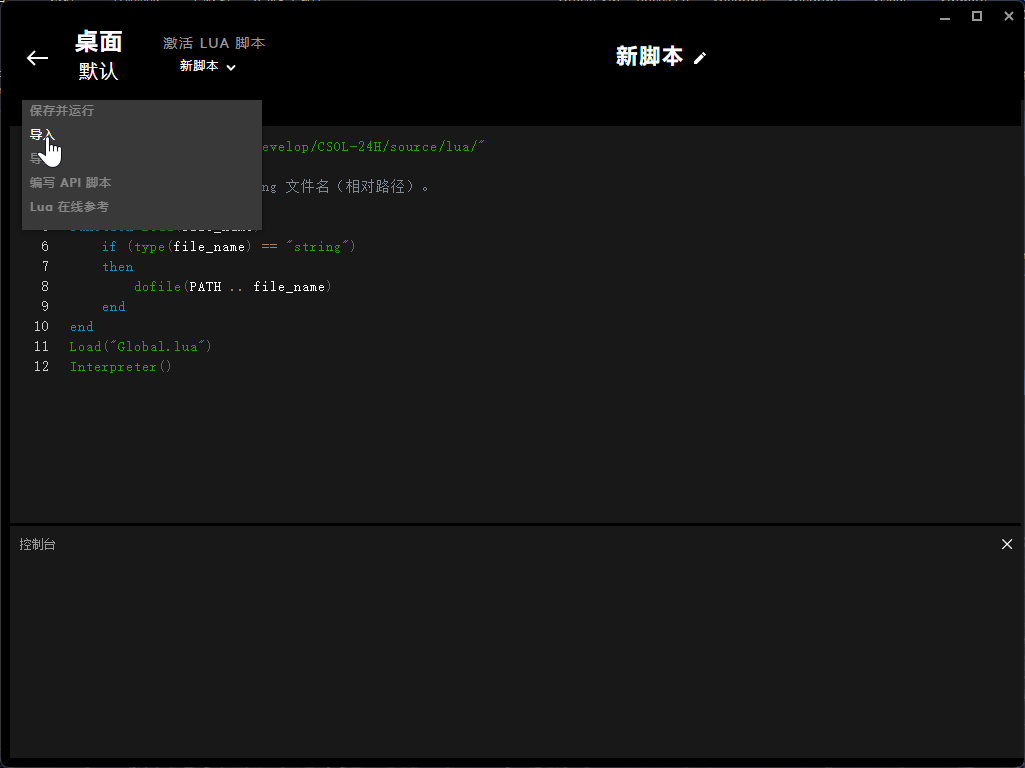
\includegraphics[width=\textwidth]{docs/assets/import.png}
    \caption{点击“导入”}
\end{figure}

\begin{figure}[H]
    \Centering
    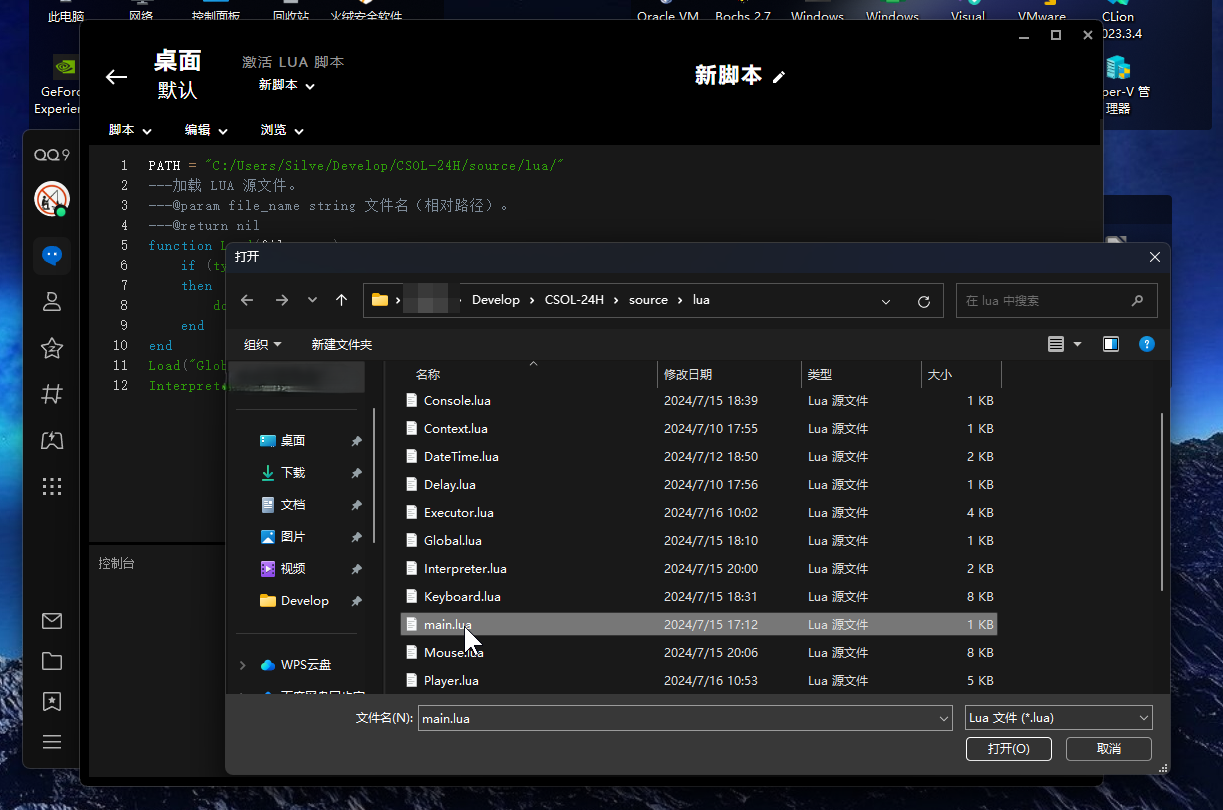
\includegraphics[width=\textwidth]{docs/assets/main.png}
    \caption{选择 \lstinline{main.lua}}
\end{figure}

看到控制台输出下述文字信息,则说明导入成功。后续若对文件夹内的 LUA 源文件进行修改,则还需要重新在此界面中保存并运行。

\begin{figure}[H]
    \Centering
    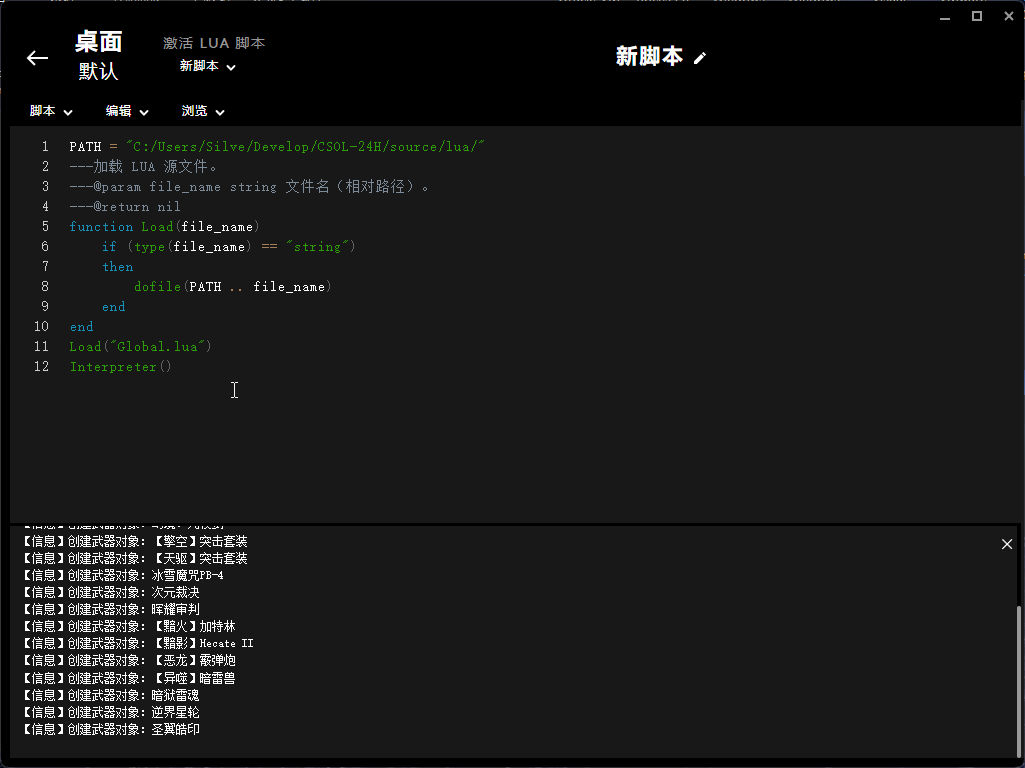
\includegraphics[width=\textwidth]{docs/assets/success.png}
    \caption{保存并运行成功}
\end{figure}

\subsection{即时中断功能}

为实现较为精确的定时控制,控制器在下达命令时均会附带一个时间戳,LUA 程序会据此验证此命令是否过期。
对于与挂机相关的命令,一旦时间差达到 5 秒,则认为下达的命令无效,不会执行相应的命令。
因此,LUA 程序中的时区信息必须配置正确(参见第 3 节)。
此外,每条命令的执行完毕都需要一定的时间。
\textbf{因此,控制器切换模式不会立即停止当前命令的执行,而是有一定的延迟时间。}

为了使罗技软件能够即时相应中断消息,本集成工具通过封装罗技 API,在 LUA 模块中引入了即时中断功能。

例如,若不慎错误地按下前面提及的功能热键,导致鼠标键盘不受控制,可以同时按下键盘上的左 \lstinline{Ctrl} 和右 \lstinline{Ctrl} 紧急暂停,罗技软件会在 10 毫秒内响应此中断信号。
紧急暂停后,罗技软件将不再发出任何键鼠操作,直至同时按下键盘上的左 \lstinline{Alt} 和右 \lstinline{Alt} 恢复。

相应地,您可以在罗技软件控制台中看到相应的提示信息。

\begin{figure}[H]
    \Centering
    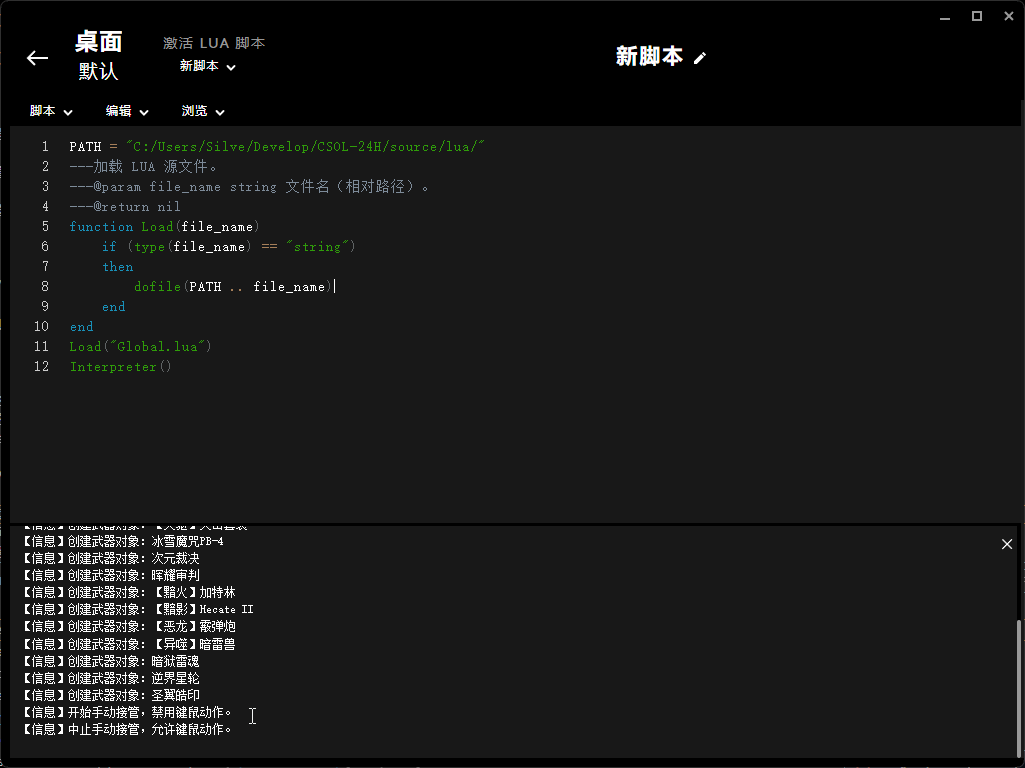
\includegraphics[width=\textwidth]{docs/assets/interrupt.png}
    \caption{即时中断功能提示信息}
\end{figure}

需要注意,紧急暂停功能完全独立于控制器。
紧急暂停后,控制器仍然会持续向罗技软件下达命令,只是罗技软件并不会执行这些命令,若要取消当前启用的功能,请按热键将控制器切换回 0 模式。

\subsection{关于更新}

\lstinline{lua} 目录下的 \lstinline{Setting.lua} 及 \lstinline{WeaponList.lua} 按照本文档介绍的方式配置完毕,能够正常使用后,应当妥善保管。
后续更新不会对这两个配置文件内容作出较大的变动。更新到新版本时,一般只需要将这两份文件原样复制到新版本的 \lstinline{lua} 目录下,并在新版本目录下重新运行一次 \lstinline{install.ps1} 即可。